\documentclass{beamer}
\usepackage{url}
\usepackage{hyperref}
\usepackage{listings}
\usepackage{booktabs}
\usepackage{tikz}
\usepackage{fontawesome5}
\usepackage{textcomp}
\usepackage{xcolor}

\usetheme{utk}

% ── Custom callout commands ──
\newcommand{\livedemo}[1]{\begin{alertblock}{\faDesktop\ \textbf{Live Demo}}#1\end{alertblock}}
\newcommand{\desktoptip}[1]{\begin{block}{\faMousePointer\ Desktop Equivalent}#1\end{block}}

% ── Listings style for bash/code blocks ──
\definecolor{codebg}{RGB}{245, 245, 245}
\definecolor{codegreen}{RGB}{0, 128, 0}
\definecolor{codegray}{RGB}{100, 100, 100}
\definecolor{codeblue}{RGB}{0, 0, 180}

\lstset{
  basicstyle=\ttfamily\scriptsize,
  backgroundcolor=\color{codebg},
  frame=single,
  framerule=0pt,
  breaklines=true,
  breakatwhitespace=true,
  columns=fullflexible,
  keepspaces=true,
  showstringspaces=false,
  commentstyle=\color{codegreen},
  keywordstyle=\color{codeblue},
  stringstyle=\color{codegray},
  xleftmargin=4pt,
  xrightmargin=4pt,
  aboveskip=6pt,
  belowskip=4pt,
}

\lstdefinelanguage{bash}{
  morekeywords={git, ssh, echo, mkdir, cd, eval, brew, sudo, apt, cat, pip, python, pbcopy, clip},
  morecomment=[l]{\#},
  morestring=[b]",
  morestring=[b]',
}

\lstdefinelanguage{yaml}{
  morekeywords={name, on, push, pull_request, branches, jobs, runs-on, steps, uses, with, run},
  morecomment=[l]{\#},
  morestring=[b]",
  morestring=[b]',
}

% ── Title info ──
\title[Git Workshop - JT:]{Git \& GitHub}
% \subtitle{A Hands-On Workshop for Industrial Engineers}
\author{Jose Tupayachi}
\institute{Department of Industrial \& Systems Engineering --- UTK}
\date{\today}
\setbeameroption{show notes on second screen=right}
\begin{document}

% ============================================================
%  TITLE SLIDE
% ============================================================
\begin{frame}
\titlepage
\end{frame}


\note{
\begin{itemize}
    \item Today we'll talk about Git and GitHub
    \item Essential tools for version control and collaboration
    \item Used in most modern software and research projects
\end{itemize}
}

% ============================================================
%  AGENDA
% ============================================================
\begin{frame}
\frametitle{Agenda}
\begin{table}[h]
\centering
\scriptsize
\begin{tabular}{clc}
\toprule
\textbf{Part} & \textbf{Topic}  \\
\midrule
1 & Setup \& Installation \\
2 & Git Basics --- Your First Repo \\
3 & Working with GitHub Remotes  \\
4 & Branching \& Merging \\
5 & Collaboration --- Pull Requests \& Code Review  \\
6 & Best Practices  \\
\bottomrule
\end{tabular}
\end{table}
% \vspace{4mm}
% \textbf{Total:} $\sim$2 hours \hfill \textbf{Level:} Beginner to Intermediate


\vspace{2mm}
\small\textit{We'll cover both the \textbf{command line} and \textbf{GitHub Desktop} (GUI) for every workflow, with live demos throughout.}
\end{frame}
\note{
\begin{itemize}
    \item first of all ill be covering the setup and installation
    \item then we will cover git basics --- creating a repo, making commits, viewing history, undoing changes, and using .gitignore
    \item next we will connect our local repo to GitHub, push and pull changes, and discuss the difference between cloning, forking, and creating cloud repos
    \item after that we will dive into branching and merging --- creating branches, working on them, and merging back to main
    \item then we will cover collaboration workflows --- how to contribute to other people's projects using pull requests and code reviews
    \item finally we will wrap up with some best practices for using Git in your day-to-day projects
\end{itemize}

}



% ============================================================
%  WHY VERSION CONTROL?
% ============================================================
\begin{frame}
\frametitle{Why Version Control?}
\textbf{The Problem (sound familiar?):}
\begin{itemize}
    \item \texttt{simulation\_model\_final.py}
    \item \texttt{simulation\_model\_final\_v2.py}
    \item \texttt{simulation\_model\_FINAL\_really\_final.py}
    \item ``Which version of the optimization script has the latest constraints?''
    \item ``Who changed the demand forecast parameters and when?''
    \item ``I broke the scheduling model --- how do I go back?''
\end{itemize}
\vspace{4mm}
\textbf{The Solution: Git}
\begin{itemize}
    \item Track every change to your scripts, data pipelines, and reports
    \item Revert to any previous state instantly
    \item Collaborate on team projects without overwriting each other's work
\end{itemize}
\end{frame}

\note{
\begin{itemize}
    \item Many file versions --- hard to manage
    \item Not clear which is the latest
    \item Hard to track who changed what
    \item Hard to undo mistakes
    \item Git tracks line-by-line changes
    \item We can go back to any older version instantly
    \item Teamwork becomes much easier
\end{itemize}
}


% ============================================================
%  GIT vs GITHUB
% ============================================================
\begin{frame}
\frametitle{Git vs.\ GitHub}
\begin{table}[h]
\centering
\small
\begin{tabular}{ll}
\toprule
\textbf{Git} & \textbf{GitHub} \\
\midrule
Version control tool & Cloud hosting platform \\
Runs locally & Accessible from anywhere \\
Command-line based & Web interface + API \\
Free \& open source & Free tier + paid plans \\
\bottomrule
\end{tabular}
\end{table}
\vspace{4mm}
\begin{block}{Analogy}
\textbf{Git} is like a camera (takes snapshots). \\
\textbf{GitHub} is like a photo album in the cloud (stores \& shares them).
\end{block}
\end{frame}

\note{
\begin{itemize}
    \item Git and GitHub are not the same thing
    \item Git is the version control system that runs locally on your computer
    \item GitHub is a cloud platform that hosts Git repositories
    \item Other platforms: GitLab, Bitbucket, Azure DevOps --- same Git commands, different hosts
\end{itemize}
}

% %%%%%%%%%%%%%%%%%%%%%%%%%%%%%%%%%%%%%%%%%%%%%%%%%%%%%%%%%%%%
%  PART 1: SETUP & INSTALLATION
% %%%%%%%%%%%%%%%%%%%%%%%%%%%%%%%%%%%%%%%%%%%%%%%%%%%%%%%%%%%%
\section{Part 1: Setup \& Installation}




% ── GitHub Account ──
\begin{frame}
\frametitle{Prerequisites: Creating a GitHub Account}
\begin{enumerate}
    \item Go to \url{https://github.com}
    \item Click \textbf{Sign Up}
    \item Choose a username, enter your email, create a password
    \item Verify your email address
\end{enumerate}
\vspace{4mm}
\end{frame}

\note{
\begin{itemize}
    \item Everyone needs a GitHub account to follow along
    \item Go to github.com and sign up if you don't have one
    \item It's free and only takes a minute
\end{itemize}
}


\begin{frame}
\frametitle{Part 1: Setup \& Installation}
\centering
\Large \textbf{Setup \& Installation}\\[6pt]
% \normalsize Duration: $\sim$15 minutes
\end{frame}

% ── Installing Git ──
\begin{frame}[fragile]
\frametitle{1.1 Installing Git (command line)}

\textbf{macOS} (usually pre-installed):
\begin{lstlisting}[language=bash]
git --version
# or install via Homebrew:
brew install git
\end{lstlisting}

\textbf{Windows:}
\begin{itemize}
    \item Download from \url{https://git-scm.com/download/win}
    % \item Run installer with defaults --- includes \textbf{Git Bash}
\end{itemize}

\textbf{Linux (Ubuntu/Debian):}
\begin{lstlisting}[language=bash]
sudo apt update && sudo apt install git
\end{lstlisting}
\end{frame}

\note{
\begin{itemize}
    \item macOS: install Homebrew first from \url{https://brew.sh}
    \item Windows: open PowerShell with admin rights before installing
    \item Windows: install Chocolatey from \url{https://chocolatey.org/install}
\end{itemize}
}

% ── Configuring Git ──
\begin{frame}[fragile]
\frametitle{1.2 Configuring Git}

Set your identity (attached to every commit):
\begin{lstlisting}[language=bash]
git config --global user.name "Your Name"
git config --global user.email "your.email@example.com"
\end{lstlisting}

Set default branch name:
\begin{lstlisting}[language=bash]
git config --global init.defaultBranch main
\end{lstlisting}

% Set default editor (optional):
% \begin{lstlisting}[language=bash]
% # VS Code
% git config --global core.editor "code --wait"
% # nano / vim
% git config --global core.editor "nano"
% \end{lstlisting}

Verify:
\begin{lstlisting}[language=bash]
git config --list
\end{lstlisting}
\end{frame}


% ── SSH Key Setup ──
\begin{frame}[fragile]
\frametitle{1.4 SSH Key Authentication (Recommended)}

\textbf{Step 1 --- Generate a key:}
\begin{lstlisting}[language=bash]
ssh-keygen -t ed25519 -C "your.email@example.com"
\end{lstlisting}

% 

\textbf{Step 2 --- Copy public key:}
\begin{lstlisting}[language=bash]
cat ~/.ssh/id_ed25519.pub         # Linux/macOS (copy manually)
\end{lstlisting}

\textbf{Step 3 --- Add to GitHub:}\\
Settings $\rightarrow$ SSH keys $\rightarrow$ New SSH key $\rightarrow$ Paste

\textbf{Step 4 --- Test:}
\begin{lstlisting}[language=bash]
ssh -T git@github.com
\end{lstlisting}
\end{frame}
\note{
\begin{itemize}
    \item Step 3b (Rarely needed): Start the SSH agent and add the key
    \item \texttt{eval "\$(ssh-agent -s)"}
    \item \texttt{ssh-add \textasciitilde/.ssh/id\_ed25519}
\end{itemize}
}

% ── GitHub Desktop Tools ──
\begin{frame}
\frametitle{1.5 GitHub Desktop (Desktop GUI)}

\vspace{4mm}
\textbf{Install GitHub Desktop now:} \url{https://desktop.github.com}
\begin{itemize}
    \item Sign in with your GitHub account
    \item It auto-configures your Git identity
\end{itemize}
\end{frame}

\note{
\begin{itemize}
    \item GitHub Desktop simplifies Git with a visual interface
    \item No need to manually configure remotes or stage files from the terminal
    \item Use buttons and checkboxes instead of typing commands
\end{itemize}
}

% ── Exercise 1 ──
\begin{frame}
\frametitle{Exercise 1}
\begin{enumerate}
    \item Verify Git is installed: \texttt{git - -version}
    \item Configure your name and email with \texttt{git config}
    \item Create a GitHub account (if you don't have one)
    \item \textbf{Install GitHub Desktop} from \url{https://desktop.github.com}
    \item Set up SSH key authentication (not needed for GitHub Desktop)
    \item Test with \texttt{ssh -T git@github.com}
\end{enumerate}
\livedemo{I'll walk through this setup on my machine right now.}
\end{frame}


\note{
\begin{itemize}
    \item GitHub Desktop emulates all the same functionality as the terminal
    \item Great for visualizing changes before committing
\end{itemize}
}
% %%%%%%%%%%%%%%%%%%%%%%%%%%%%%%%%%%%%%%%%%%%%%%%%%%%%%%%%%%%%
%  PART 2: GIT BASICS
% %%%%%%%%%%%%%%%%%%%%%%%%%%%%%%%%%%%%%%%%%%%%%%%%%%%%%%%%%%%%
\section{Part 2: Git Basics}

\begin{frame}
\frametitle{Part 2: Git Repos}
\centering
\Large \textbf{Git Repos --- First Repository}\\[6pt]
% \normalsize Duration: $\sim$25 minutes
\end{frame}




% ── Key Concepts ──
\begin{frame}
\frametitle{2.1 What Is Git? --- Key Concepts}

Git is a \textbf{distributed version control system} --- an unlimited undo history for your project.

\vspace{4mm}
\begin{center}
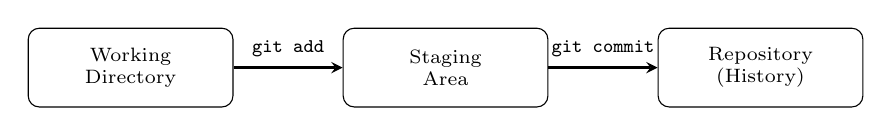
\begin{tikzpicture}[
    box/.style={draw, rounded corners, minimum width=2.6cm, minimum height=1cm, align=center, font=\scriptsize},
    arr/.style={->, thick, >=stealth}
]
\node[box] (wd) at (0,0) {Working\\Directory};
\node[box] (sa) at (4,0) {Staging\\Area};
\node[box] (repo) at (8,0) {Repository\\(History)};
\draw[arr] (wd) -- node[above, font=\scriptsize]{\texttt{git add}} (sa);
\draw[arr] (sa) -- node[above, font=\scriptsize]{\texttt{git commit}} (repo);
\end{tikzpicture}
\end{center}

\vspace{4mm}
\begin{table}[h]
\centering
\scriptsize
\begin{tabular}{ll}
\toprule
\textbf{Concept} & \textbf{Description} \\
\midrule
Repository (repo) & A project folder tracked by Git \\
Commit & A snapshot at a point in time \\
Staging Area & Preparation zone for the next commit \\
Working Directory & The actual files on your computer \\
\bottomrule
\end{tabular}
\end{table}
\end{frame}

% ── Creating a Repo ──
\begin{frame}[fragile]
\frametitle{2.2 Creating Your First Repository}

\textbf{Command Line:}
\begin{lstlisting}[language=bash]
# Create a project folder
mkdir ie-supply-chain
cd ie-supply-chain

# Initialize Git tracking
git init
\end{lstlisting}

\desktoptip{File $\rightarrow$ New Repository $\rightarrow$ choose name \& folder $\rightarrow$ Create Repository}

\vspace{2mm}
Check the status (you will use this \textbf{constantly}):
\begin{lstlisting}[language=bash]
git status
\end{lstlisting}
\end{frame}

\note{
\begin{itemize}
    \item Run \texttt{ls -a} to show the hidden \texttt{.git} folder
    \item Check status with \texttt{git status}
    \item Also show how to import the repo in GitHub Desktop
\end{itemize}
}

% ── Creating a Repo via GitHub Desktop ──
\begin{frame}
\frametitle{2.2a Creating a Repo from GitHub Desktop}

\textbf{Step-by-step in GitHub Desktop:}
\begin{enumerate}
    \item Open GitHub Desktop
    \item Go to \textbf{File} $\rightarrow$ \textbf{New Repository\ldots}
    \item Fill in:
    \begin{itemize}
        \item \textbf{Name:} \texttt{ie-supply-chain}
        \item \textbf{Local Path:} choose where to save it
        \item (Optional) check \textbf{Initialize this repository with a README}
        \item (Optional) pick a \textbf{.gitignore} template (e.g.\ Python)
    \end{itemize}
    \item Click \textbf{Create Repository}
\end{enumerate}

\vspace{2mm}
GitHub Desktop creates the folder, runs \texttt{git init}, and opens the repo --- no terminal needed.

\vspace{2mm}
\textbf{To open the folder in your editor:}\\
Repository $\rightarrow$ Open in \textit{Visual Studio Code} (or your default editor)
\end{frame}

\note{
\begin{itemize}
    \item Point out the \textbf{Current Repository} dropdown in the top-left --- that's how you switch between repos
    \item The \textbf{No local changes} message confirms the repo is clean right after creation
    \item Show the \textbf{History} tab --- it already has one commit if README was checked
\end{itemize}
}

% ── Creating a Repo on GitHub and Cloning ──
\begin{frame}[fragile]
\frametitle{2.2b Creating a Cloud Repo \& Cloning Locally}

\textbf{Step 1 --- Create the repo on GitHub:}
\begin{enumerate}
    \item Go to \url{https://github.com/new}
    \item Enter a name, choose Public or Private
    \item Check \textbf{Add a README file} (and optionally a .gitignore)
    \item Click \textbf{Create repository}
\end{enumerate}

\vspace{2mm}
\textbf{Step 2 --- Clone it to your machine:}
\begin{lstlisting}[language=bash]
# SSH (recommended)
git clone git@github.com:USERNAME/ie-supply-chain.git

\end{lstlisting}

\desktoptip{On GitHub click \textbf{Code} $\rightarrow$ \textbf{Open with GitHub Desktop} --- it clones and opens automatically.}

\vspace{1mm}
\small This gives you a local copy \emph{already connected} to the remote --- no \texttt{git remote add} needed.
\end{frame}

\note{
\begin{itemize}
    \item This is the \textbf{easiest starting point} for new projects --- create on GitHub first, then clone
    \item The clone command sets up the \texttt{origin} remote automatically
    \item Difference from 2.2: here GitHub is the source of truth; in 2.2 the local folder is
    \item Show the \textbf{Code} button on GitHub and the clone URL options (SSH vs HTTPS)
\end{itemize}
}

% ── The Git Workflow ──
\begin{frame}[fragile]
\frametitle{2.3 The Git Workflow: Add $\rightarrow$ Commit }
\texttt{not staged | not committed}\\
\textbf{Command Line:}
\begin{lstlisting}[language=bash]
# Step 1: Create a file
echo "# Supply Chain Analysis" > README.md

# Step 2: Stage the file
git add README.md

# Step 3: Commit
git commit -m "Initial commit: add README"
\end{lstlisting}

\desktoptip{Changed files appear in the left panel. Check the boxes to stage, type a commit message at the bottom, click \textbf{Commit to main}.}

\livedemo{GitHub Desktop side by side add and commit}
\end{frame}

\note{
\begin{itemize}
    \item Install VS Code on Windows: \texttt{choco install vscode}
    \item Install Python 3 on Windows: \texttt{choco install python310}
    \item After installing Python on Windows, disable ``App execution aliases'' in Settings
    \item Windows: use \texttt{python}; Linux/macOS: use \texttt{python3}
    
    \item also we can load the repo to github desktop we can link it
    
    \item for the live demo "desktop" we can create a new  repo from github desktop too! Create a new repo
\end{itemize}
}

% ── Viewing Changes ──
\begin{frame}[fragile]
\frametitle{2.4 Making Changes \& Viewing Diffs}

\textbf{Command Line:}
\begin{lstlisting}[language=bash]
# Edit the file
echo "## About" >> README.md
echo "Supply chain optimization project." >> README.md

# See what changed
git diff            # exact line-by-line changes (before adding changes)
\end{lstlisting}

\texttt{git diff} output: lines with \texttt{+} were \textbf{added}, lines with \texttt{-} were \textbf{removed}.

\begin{lstlisting}[language=bash]
git add README.md
git commit -m "Add About section to README"
\end{lstlisting}

\desktoptip{Click any changed file to see a \textbf{visual diff} (green/red highlighting). No commands needed!}
\end{frame}

% ── Viewing History ──
\begin{frame}[fragile]
\frametitle{2.5 Viewing History}

\textbf{Command Line:}
\begin{lstlisting}[language=bash]
git log                         # full commit log
git log --oneline               # compact view
git log --oneline --graph --all # graphical view
git show <commit-hash>          # specific commit
\end{lstlisting}

\desktoptip{Click the \textbf{History} tab to see all commits with diffs, authors, and timestamps in a visual timeline.}
\end{frame}

% ── Undoing Things ──
\begin{frame}[fragile]
\frametitle{2.6 Undoing Things}

% \textbf{Command Line:}
\begin{lstlisting}[language=bash]

# You staged "added ." a file but changed your mind -- unstage it (keep your edits take it out of the added files)
git restore --staged analysis.py

# You edited a file and want to throw away all changes (go back to last commit, or simply remove changes for that file)
git restore analysis.py             # WARNING: permanent, edits are gone! What was modified will be removed

# You just committed but the message has a typo
git commit --amend -m "feat: add demand forecast (corrected)" # if nothing added it will just change the name of what was committed

git add analysis.py
git commit --amend --no-edit       # rewrites last commit to include analysis.py, you can use a new message or simply no edit to keep the same message
\end{lstlisting}
\tiny
\desktoptip{Right-click a file $\rightarrow$ \textbf{Discard Changes}. To amend: check \textbf{Amend commit} at the bottom of the commit panel before clicking Commit.}
\end{frame}


\note{\# You just committed but forgot to include a file you already edited
\# (only works if you have NOT pushed yet, or else you have to do a new commit and re push)}


% ── .gitignore ──
\begin{frame}[fragile]
\frametitle{2.7 The .gitignore File}

Tells Git which files to \textbf{never track}. Create a file called \texttt{.gitignore} in your repo root:
\tiny
\begin{lstlisting}
    
# Compiled / generated files
*.pyc
__pycache__/

# OS files
.DS_Store
Thumbs.db

# IDE files
.vscode/
.idea/

# Large data (track with Git LFS instead)
*.csv
*.xlsx
data/raw/

# Secrets & environment
.env
*.key
\end{lstlisting}
\end{frame}

% ── .gitignore Patterns Tutorial ──
\begin{frame}[fragile]
\frametitle{2.7b .gitignore --- Pattern Cheat Sheet}

\begin{table}[h]
\centering
\tiny
\begin{tabular}{lll}
\toprule
\textbf{Pattern} & \textbf{Matches} & \textbf{Example} \\
\midrule
\texttt{*.csv} & All CSV everywhere & \texttt{sales.csv} \\
\texttt{build/} & Directory (1 hop) & \texttt{build/model.pkl} \\
\texttt{data/} & Directory (even innner dirs) & \texttt{data/raw/file.txt} \\

\texttt{!data/README.md} & Exception & keep one file \\
\texttt{*.log} & Log files & \texttt{run.log} \\

\texttt{**/*.tmp} & Any Temp file & \texttt{src/a/b.tmp} \\
\bottomrule
\end{tabular}
\end{table}

\vspace{2mm}
\textbf{Auto-generate a starter \texttt{.gitignore}:}
\begin{lstlisting}[language=bash]
# Use gitignore.io (now toptal.com)
curl -sL "https://www.toptal.com/developers/gitignore/api/\
python,macos,windows,visualstudiocode" > .gitignore
\end{lstlisting}

Or browse templates at \url{https://github.com/github/gitignore}
\end{frame}

% ── Three States Diagram ──
\begin{frame}
\frametitle{2.8 Understanding the Three States}

\begin{center}
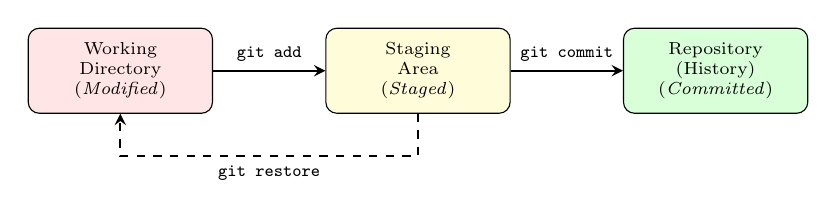
\begin{tikzpicture}[
    scale=0.9,
    transform shape,
    box/.style={draw, rounded corners, minimum width=2.6cm, minimum height=1.2cm, align=center, font=\scriptsize},
    arr/.style={->, thick, >=stealth}
]
\node[box, fill=red!10] (wd) at (0,0) {Working\\Directory\\(\textit{Modified})};
\node[box, fill=yellow!15] (sa) at (4.2,0) {Staging\\Area\\(\textit{Staged})};
\node[box, fill=green!15] (repo) at (8.4,0) {Repository\\(History)\\(\textit{Committed})};
\draw[arr] (wd) -- node[above, font=\scriptsize]{\texttt{git add}} (sa);
\draw[arr] (sa) -- node[above, font=\scriptsize]{\texttt{git commit}} (repo);
\draw[arr, dashed] (sa.south) -- ++(0,-0.6) -| node[below, near start, font=\scriptsize]{\texttt{git restore}} (wd.south);
\end{tikzpicture}
\end{center}

\vspace{2mm}
\begin{table}[h]
\centering
\scriptsize
\begin{tabular}{lll}
\toprule
\textbf{State $t_0$} & \textbf{Description} & \textbf{Next Command $t_1$} \\
\midrule
Modified & Not staged & \texttt{git add} \\
Staged & Ready to commit & \texttt{git commit} \\
Committed & In history & --- \\
\bottomrule
\end{tabular}
\end{table}
\end{frame}

% ── Exercise 2a ──
\begin{frame}
\frametitle{Exercise 2 --- Part A}
\textbf{Try both the command line AND GitHub Desktop:}
\begin{enumerate}
    \item Create a new folder \texttt{ie-project} and initialize a Git repo
    \item Create at least 3 files (e.g., \texttt{README.md}, \texttt{analysis.py}, \texttt{.gitignore})
    \item Make an initial commit with all files
    \item Edit \texttt{analysis.py} and view the diff
    \item Make a second commit
    \item View your history with \texttt{git log --oneline} (or the History tab)
\end{enumerate}
\vspace{2mm}
\livedemo{I'll do this exercise live --- terminal on the left, GitHub Desktop on the right.}
\end{frame}

% ── Exercise 2b ──
\begin{frame}[fragile]
\frametitle{Exercise 2 --- Part B: Staging \& Restore}
\textbf{Practice undoing things (command line):}
\begin{enumerate}
    \item Edit \texttt{analysis.py} --- then \textbf{stage} it with \texttt{git add}
    \item Change your mind: \textbf{unstage} it (keep your edits on disk)
    \begin{lstlisting}[language=bash]
git restore --staged analysis.py
    \end{lstlisting}
    \item Edit \texttt{analysis.py} again --- this time \textbf{discard} all changes entirely
    \begin{lstlisting}[language=bash]
git restore analysis.py     # WARNING: edits are gone!
    \end{lstlisting}
    \item Make a commit, then realize the message has a typo --- fix it
    \begin{lstlisting}[language=bash]
git commit --amend -m "feat: corrected message"
    \end{lstlisting}
    \item Make a commit, then add a forgotten file to that same commit
    \begin{lstlisting}[language=bash]
git add forgotten.py
git commit --amend --no-edit
    \end{lstlisting}
\end{enumerate}
\desktoptip{Right-click a file $\rightarrow$ \textbf{Discard Changes} to restore. Check \textbf{Amend commit} before clicking Commit to amend.}
\end{frame}

% %%%%%%%%%%%%%%%%%%%%%%%%%%%%%%%%%%%%%%%%%%%%%%%%%%%%%%%%%%%%
%  PART 3: GITHUB REMOTES
% %%%%%%%%%%%%%%%%%%%%%%%%%%%%%%%%%%%%%%%%%%%%%%%%%%%%%%%%%%%%
\section{Part 3: Working with GitHub Remotes}

\begin{frame}
\frametitle{Part 3: GitHub Remotes}
\centering
\Large \textbf{Working with GitHub Remotes}\\[6pt]
% \normalsize Duration: $\sim$20 minutes
\end{frame}

% ── Local vs Remote ──
\begin{frame}
\frametitle{3.1 Local vs.\ Remote}

\begin{center}
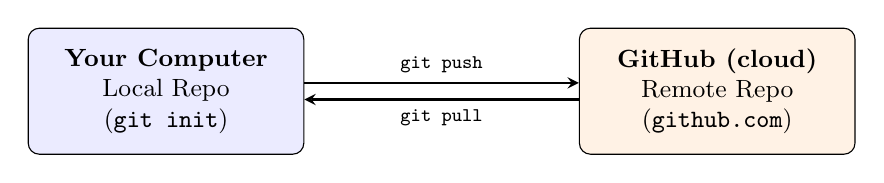
\begin{tikzpicture}[
    box/.style={draw, rounded corners, minimum width=3.5cm, minimum height=1.6cm, align=center, font=\small},
    arr/.style={->, thick, >=stealth}
]
\node[box, fill=blue!8] (local) at (0,0) {\textbf{Your Computer}\\Local Repo\\(\texttt{git init})};
\node[box, fill=orange!10] (remote) at (7,0) {\textbf{GitHub (cloud)}\\Remote Repo\\(\texttt{github.com})};
\draw[arr] ([yshift=3pt]local.east) -- node[above, font=\scriptsize]{\texttt{git push}} ([yshift=3pt]remote.west);
\draw[arr] ([yshift=-3pt]remote.west) -- node[below, font=\scriptsize]{\texttt{git pull}} ([yshift=-3pt]local.east);
\end{tikzpicture}
\end{center}

\vspace{4mm}
Other platforms: GitLab, Bitbucket, Azure DevOps --- same Git commands, different hosts.
\end{frame}

% ── Creating a Repo on GitHub ──
\begin{frame}
\frametitle{3.2 Creating a Repository on GitHub}

\textbf{Option A: Create on GitHub first}:
\begin{enumerate}
    \item Go to \url{https://github.com/new}
    \item Repository name: \texttt{ie-supply-chain}
    \item Visibility: Public or Private
    \item \textbf{Do NOT} initialize with README (we have one locally)
    \item Click \textbf{Create repository}
\end{enumerate}

\desktoptip{File $\rightarrow$ New Repository --- or Publish Repository if you already have a local repo open.}
\end{frame}

% ── Connecting & Pushing ──
\begin{frame}[fragile]
\frametitle{3.3 Connecting Local to Remote \& Pushing}

\textbf{Add a remote:}
\begin{lstlisting}[language=bash]
# SSH (recommended)
git remote add origin git@github.com:USER/ie-supply-chain.git

# HTTPS
git remote add origin https://github.com/USER/ie-supply-chain.git
\end{lstlisting}

\textbf{First push:}
\begin{lstlisting}[language=bash]
git push -u origin main
\end{lstlisting}

\desktoptip{Click \textbf{Publish Repository} (top bar). Choose public/private. Done --- no remote/URL needed!}

\livedemo{Publishing our IE project repo --- CLI and Desktop.}
\end{frame}

% ── Cloning ──
\begin{frame}[fragile]
\frametitle{3.4 Cloning a Repository}

\textbf{Command Line:}
\begin{lstlisting}[language=bash]
# SSH
git clone git@github.com:USERNAME/REPOSITORY.git

# HTTPS
git clone https://github.com/USERNAME/REPOSITORY.git
\end{lstlisting}

\desktoptip{File $\rightarrow$ Clone Repository $\rightarrow$ paste URL or pick from your GitHub repos list $\rightarrow$ Clone.}

Creates a local copy with full commit history and remote already configured.
\end{frame}

% ── Pulling Changes ──
\begin{frame}[fragile]
\frametitle{3.5 Pulling Changes}

\textbf{Command Line:}
\begin{lstlisting}[language=bash]
git pull        # fetch + merge in one step
git push        # share your changes
\end{lstlisting}

\desktoptip{Click \textbf{Fetch Origin} (top bar) to check for updates, then \textbf{Pull Origin} to download them. Click \textbf{Push Origin} to upload your commits.}

\vspace{2mm}
\textbf{The Push/Pull Workflow:}
\begin{enumerate}
    \item Make changes locally
    \item \texttt{git pull} \hfill $\leftarrow$ get latest first
    \item \texttt{git add .} \& \texttt{git commit -m "description"}
    \item \texttt{git push} \hfill $\leftarrow$ share your changes
\end{enumerate}

% \begin{block}{Golden Rule}
\textcolor{red}{Always \texttt{pull} before you \texttt{push} to minimize merge conflicts.}
% \end{block}
\end{frame}

% ── Clone vs Fork vs Create ──
\begin{frame}
\frametitle{3.6 Clone vs.\ Fork vs.\ Create}
\begin{table}[h]
\centering
\small
\begin{tabular}{lll}
\toprule
\textbf{Action} & \textbf{When to use} & \textbf{Command} \\
\midrule
Create & New project & \texttt{git init} + \texttt{remote add} \\
Clone & Repo you have access to & \texttt{git clone <url>} \\
Fork & Someone else's project & Fork on GitHub, then clone \\
\bottomrule
\end{tabular}
\end{table}
\end{frame}

% ── Exercise 3 ──
\begin{frame}
\frametitle{Exercise 3}
\textbf{Pick your tool: Command Line or GitHub Desktop (or both!):}
\begin{enumerate}
    \item Create a new repository on GitHub
    \item Connect and push your local repo (CLI: \texttt{git remote add} + \texttt{push} / Desktop: \textbf{Publish Repository})
    \item Verify your files appear on GitHub
    \item Edit a file on GitHub directly (pencil icon), commit it
    \item Pull the changes locally (CLI: \texttt{git pull} / Desktop: \textbf{Fetch} then \textbf{Pull})
\end{enumerate}
\livedemo{Pushing and pulling --- showing both workflows on the same repo.}
\end{frame}

% %%%%%%%%%%%%%%%%%%%%%%%%%%%%%%%%%%%%%%%%%%%%%%%%%%%%%%%%%%%%
%  PART 4: BRANCHING & MERGING
% %%%%%%%%%%%%%%%%%%%%%%%%%%%%%%%%%%%%%%%%%%%%%%%%%%%%%%%%%%%%
\section{Part 4: Branching \& Merging}

\begin{frame}
\frametitle{Part 4: Branching \& Merging}
\centering
\Large \textbf{Branching \& Merging}\\[6pt]
% \normalsize Duration: $\sim$20 minutes
\end{frame}

% ── What Are Branches ──
\begin{frame}
\frametitle{4.1 What Are Branches?}

Branches = \textbf{parallel timelines} for your project.

\begin{center}
\begin{tikzpicture}[
    commit/.style={circle, draw, fill=Smokey, minimum size=6pt, inner sep=0pt},
    commitO/.style={circle, draw, fill=TennesseeOrange, minimum size=6pt, inner sep=0pt},
]
% main branch
\node[commit] (m1) at (0,0) {};
\node[commit] (m2) at (1.5,0) {};
\node[commit] (m3) at (3,0) {};
\node[commit] (m4) at (6,0) {};
\node[commit] (m5) at (7.5,0) {};

% feature branch
\node[commitO] (f1) at (3,1) {};
\node[commitO] (f2) at (4.5,1) {};

\draw[thick] (m1) -- (m2) -- (m3);
\draw[thick] (m4) -- (m5);
\draw[thick, TennesseeOrange] (m2) -- (f1) -- (f2);
\draw[thick, TennesseeOrange] (f2) -- (m4);
\draw[thick] (m3) -- (m4);

\node[above right, font=\scriptsize, TennesseeOrange] at (f1) {feature-branch};
\node[below, font=\scriptsize] at (m1) {main};
\node[above, font=\scriptsize] at (m4) {merge};
\end{tikzpicture}
\end{center}

\vspace{4mm}
\begin{itemize}
    \item Develop features without breaking \texttt{main}
    \item Experiment freely --- throw away if it doesn't work
    \item Multiple people work on different things simultaneously
\end{itemize}
\end{frame}

% ── Creating and Switching Branches ──
\begin{frame}[fragile]
\frametitle{4.2 Creating \& Switching Branches}

\textbf{Command Line:}
\begin{lstlisting}[language=bash]
# See current branch
git branch

# Create AND switch in one step
git switch -c feature/demand-forecast
\end{lstlisting}

\textbf{Legacy alternative:} \texttt{git checkout -b feature/demand-forecast}

\desktoptip{Branch $\rightarrow$ New Branch $\rightarrow$ type name $\rightarrow$ Create Branch. Switching: click the \textbf{Current Branch} dropdown and select.}

\livedemo{Creating and switching branches in both tools.}
\end{frame}

% ── Working on a Branch ──
\begin{frame}[fragile]
\frametitle{4.3 Working on a Branch}

\textbf{Command Line:}
\begin{lstlisting}[language=bash]
# 1. Create and switch to a new branch
git switch -c feature/demand-forecast

# 2. Make changes
echo "def forecast_demand(history):" > forecast.py
echo "    return sum(history) / len(history)" >> forecast.py

# 3. Stage and commit
git add forecast.py
git commit -m "feat: add demand forecast function"

# 4. View branch history
git log --oneline --graph --all
\end{lstlisting}

\desktoptip{Edit files in your editor. Changes auto-appear in Desktop's left panel. Write message $\rightarrow$ \textbf{Commit to feature/demand-forecast}.}
\end{frame}

% ── Merging Branches ──
\begin{frame}[fragile]
\frametitle{4.4 Merging Branches}

\textbf{Command Line:}
\begin{lstlisting}[language=bash]
# Step 1: Switch to the target branch
git switch main

# Step 2: Merge the feature branch
git merge feature/demand-forecast

# Step 3: Delete the branch (cleanup)
git branch -d feature/demand-forecast
\end{lstlisting}

\desktoptip{Switch to \texttt{main} via the branch dropdown. Then Branch $\rightarrow$ \textbf{Merge into Current Branch} $\rightarrow$ select the feature branch.}

\vspace{2mm}
\begin{table}[h]
\centering
\scriptsize
\begin{tabular}{lll}
\toprule
\textbf{Type} & \textbf{When} & \textbf{Result} \\
\midrule
Fast-forward & No new commits on \texttt{main} & Linear history \\
Three-way merge & Both branches have commits & Merge commit created \\
\bottomrule
\end{tabular}
\end{table}
\end{frame}

% ── Handling Merge Conflicts ──
\begin{frame}[fragile]
\frametitle{4.5 Handling Merge Conflicts}

Conflicts happen when \textbf{two branches modify the same lines}.

\vspace{1mm}
What a conflict looks like:
\begin{lstlisting}
<<<<<<< HEAD
Hello from Main
=======
Hello from Branch A
>>>>>>> branch-a
\end{lstlisting}

\small\textbf{Resolution:} Edit the file, remove conflict markers, then stage and commit.\vspace{1mm}

\small VS Code shows ``Accept Current'', ``Accept Incoming'', ``Accept Both'' buttons.
\end{frame}

% ── Branch Naming Conventions ──
\begin{frame}
\frametitle{4.6 Branch Naming Conventions}

\begin{table}[h]
\centering
\small
\begin{tabular}{ll}
\toprule
\textbf{Prefix} & \textbf{Purpose} \\
\midrule
\texttt{feature/} & New functionality \\
\texttt{bugfix/} & Bug fixes \\
\texttt{hotfix/} & Urgent production fixes \\
\texttt{docs/} & Documentation changes \\
\texttt{refactor/} & Code restructuring \\
\texttt{test/} & Adding or modifying tests \\
\bottomrule
\end{tabular}
\end{table}

\vspace{4mm}
Examples:
\begin{itemize}
    \item \texttt{feature/demand-forecast}
    \item \texttt{bugfix/fix-inventory-calc}
    \item \texttt{docs/update-process-docs}
\end{itemize}
\end{frame}

% ── Git Flow Lite ──
\begin{frame}
\frametitle{4.7 Common Branch Workflow}

\begin{center}
\begin{tikzpicture}[
    commit/.style={circle, draw, fill=Smokey, minimum size=6pt, inner sep=0pt},
    commitO/.style={circle, draw, fill=TennesseeOrange, minimum size=6pt, inner sep=0pt},
    scale=0.9
]
% main branch
\node[commit] (m1) at (0,0) {};
\node[commit] (m2) at (2,0) {};
\node[commit] (m3) at (5,0) {};
\node[commit] (m4) at (8,0) {};

% feature-a
\node[commitO] (a1) at (1,1) {};
\node[commitO] (a2) at (2,1) {};

% feature-b
\node[commitO] (b1) at (3.5,-1) {};
\node[commitO] (b2) at (5,-1) {};

\draw[thick] (m1) -- (m2) -- (m3) -- (m4);
\draw[thick, TennesseeOrange] (m1) -- (a1) -- (a2) -- (m2);
\draw[thick, TennesseeOrange] (m2) -- (b1) -- (b2) -- (m3);

\node[below, font=\scriptsize] at (m1) {main};
\node[above, font=\scriptsize, TennesseeOrange] at (a1) {feature-a};
\node[below, font=\scriptsize, TennesseeOrange] at (b1) {feature-b};
\end{tikzpicture}
\end{center}

\vspace{2mm}
\begin{enumerate}
    \item Start from \texttt{main}
    \item Create a \texttt{feature/} branch for each task
    \item Work and commit on your feature branch
    \item Merge back to \texttt{main} when done
    \item Delete the feature branch
\end{enumerate}
\end{frame}

% ── Exercise 4 ──
\begin{frame}
\frametitle{Exercise 4}
\textbf{Try with both CLI and GitHub Desktop:}
\begin{enumerate}
    \item From \texttt{main}, create branch \texttt{feature/quality-report}
    \item Create \texttt{quality\_report.py} and make 2 commits
    \item Switch to \texttt{main}, create \texttt{scheduling.py}, commit
    \item Merge \texttt{feature/quality-report} into \texttt{main}
    \item View with \texttt{git log --oneline --graph --all} (or Desktop History)
\end{enumerate}
\vspace{2mm}
\textbf{Bonus (Conflict Practice):}
\begin{enumerate}
    \item Create two branches that edit the same line in \texttt{README.md}
    \item Merge the first (no conflict), merge the second (conflict!) and resolve it
\end{enumerate}
\livedemo{Branching, merging, and resolving a conflict --- live in both tools.}
\end{frame}

% %%%%%%%%%%%%%%%%%%%%%%%%%%%%%%%%%%%%%%%%%%%%%%%%%%%%%%%%%%%%
%  PART 5: COLLABORATION
% %%%%%%%%%%%%%%%%%%%%%%%%%%%%%%%%%%%%%%%%%%%%%%%%%%%%%%%%%%%%
\section{Part 5: Collaboration}

\begin{frame}
\frametitle{Part 5: Collaboration}
\centering
\Large \textbf{Pull Requests \& Code Review}\\[6pt]
% \normalsize Duration: $\sim$25 minutes
\end{frame}

% ── Collaboration Workflow ──
\begin{frame}
\frametitle{5.1 The Collaboration Workflow}

\begin{enumerate}
    \item Fork or clone the repository
    \item Create a feature branch
    \item Make changes and push the branch
    \item Open a \textbf{Pull Request (PR)}
    \item Team reviews and discusses
    \item Merge the PR into \texttt{main}
\end{enumerate}

\vspace{4mm}
This is how open-source projects, research labs, and engineering teams work together.

\desktoptip{GitHub Desktop has a \textbf{``Create Pull Request''} button that opens GitHub in your browser, pre-filled.}
\end{frame}

% ── Creating a PR ──
\begin{frame}[fragile]
\frametitle{5.2 Pushing a Branch \& Opening a PR}

\textbf{Push your feature branch:}
\begin{lstlisting}[language=bash]
git switch feature/quality-report
git push -u origin feature/quality-report
\end{lstlisting}

\desktoptip{Click \textbf{Push Origin} (or \textbf{Publish Branch} if it's new). Then click \textbf{Create Pull Request} --- opens GitHub in your browser.}

\vspace{1mm}
\textbf{On GitHub:}
\begin{enumerate}
    \tiny
    \item Click \textbf{``Compare \& pull request''}
    \item Fill in: Title, Description, Reviewers, Labels
    \item Click \textbf{``Create pull request''}
\end{enumerate}

\vspace{1mm}
\textbf{Good PR template:}
\begin{itemize}
    \tiny
    \item \textbf{What} --- Summary of changes
    \item \textbf{Why} --- Motivation/context
    \item \textbf{Testing} --- How you verified
\end{itemize}
\end{frame}

% ── Code Review ──
\begin{frame}
\frametitle{5.3 Code Review}

\textbf{As a Reviewer:}
\begin{enumerate}
    \item Go to PR's \textbf{``Files changed''} tab
    \item Review the diff line by line
    \item Comment on any line
    \item Submit: \textbf{Comment}, \textbf{Approve}, or \textbf{Request}
\end{enumerate}

\vspace{2mm}
\textbf{Review prefixes:}
\begin{table}[h]
\centering
\tiny
\begin{tabular}{ll}
\toprule
\textbf{Prefix} & \textbf{Meaning} \\
\midrule
\texttt{nit:} & Non-blocking suggestion \\
\texttt{question:} & Clarification \\
\texttt{blocker:} & Must fix before merge \\
\bottomrule
\end{tabular}
\end{table}
\end{frame}

% ── Merging a PR ──
\begin{frame}[fragile]
\frametitle{5.4 Merging a Pull Request}

\begin{table}[h]
\centering
\scriptsize
\begin{tabular}{lll}
\toprule
\textbf{Method} & \textbf{Description} & \textbf{When to use} \\
\midrule
Merge commit & Preserves full history & Default \\
Squash \& merge & Combines into one commit & Clean main history \\
Rebase \& merge & Replays on top of main & Linear history \\
\bottomrule
\end{tabular}
\end{table}

\vspace{2mm}
\textbf{After merging on GitHub:}
\begin{lstlisting}[language=bash]
# Click "Delete branch" on GitHub, then locally:
git switch main
git pull
git branch -d feature/quality-report
\end{lstlisting}

\desktoptip{Desktop auto-detects the merged branch. Click \textbf{Fetch/Pull}, then right-click the old branch $\rightarrow$ Delete.}
\end{frame}

% ── Working with Collaborators ──
\begin{frame}
\frametitle{5.5 Working with Collaborators}

\textbf{Adding collaborators:} Settings $\rightarrow$ Collaborators $\rightarrow$ Add people

\vspace{4mm}
\begin{table}[h]
\centering
\small
\begin{tabular}{ll}
\toprule
\textbf{Role} & \textbf{Can do} \\
\midrule
Read & View and clone \\
Triage & Manage issues and PRs (no push) \\
Write & Push to branches, merge PRs \\
Maintain & Manage repo settings \\
Admin & Full access \\
\bottomrule
\end{tabular}
\end{table}
\end{frame}

% ── Fork & PR Model ──
\begin{frame}[fragile]
\frametitle{5.6 The Fork \& Pull Request Model}

For contributing to repos you \textbf{don't own}:
\begin{enumerate}
    \item \textbf{Fork} the repository (your copy on GitHub)
    \item \textbf{Clone} your fork locally
    \item Create a \textbf{feature branch} and make changes
    \item \textbf{Push} and open a PR to the original repo
    \item Maintainers review and merge
\end{enumerate}

\vspace{2mm}
\textbf{Keeping your fork up to date:}
\begin{lstlisting}[language=bash]
git remote add upstream https://github.com/OWNER/REPO.git
git fetch upstream
git switch main
git merge upstream/main
git push origin main
\end{lstlisting}
\end{frame}

% ── GitHub Issues ──
\begin{frame}[fragile]
\frametitle{5.7 GitHub Issues \& Branch Protection}

\textbf{Issues} --- built-in task/bug tracking:
\begin{itemize}
    \item Go to Issues tab $\rightarrow$ New issue
    \item Add title, description, labels, assignees
\end{itemize}

\vspace{2mm}
\textbf{Linking PRs to issues} (auto-close on merge):
\begin{lstlisting}
Fixes #12
Closes #12
Resolves #12
\end{lstlisting}

\vspace{2mm}
\textbf{Protecting \texttt{main}:} Settings $\rightarrow$ Branches $\rightarrow$ Protection rules:
\begin{itemize}
    \item Require a pull request before merging
    \item Require approvals (1+)
    \item Require status checks to pass
    \item Do not allow force pushes
\end{itemize}
\end{frame}

% ── Exercise 5 ──
\begin{frame}
\frametitle{Exercise 5}
\textbf{Part A --- Solo PR Practice (CLI or Desktop):}
\begin{enumerate}
    \item Create a branch, make changes, push to GitHub
    \item Open a Pull Request, review ``Files changed''
    \item Merge the PR, delete the branch, pull locally
\end{enumerate}

\vspace{2mm}
\textbf{Part B --- Pair Exercise:}
\begin{enumerate}
    \item Person A creates a repo, adds Person B as collaborator
    \item Person B clones (CLI or Desktop), creates branch, opens PR
    \item Person A reviews, approves, and merges
\end{enumerate}

\livedemo{Full PR lifecycle --- from branch creation to merge, shown in Desktop \& CLI.}
\end{frame}

% %%%%%%%%%%%%%%%%%%%%%%%%%%%%%%%%%%%%%%%%%%%%%%%%%%%%%%%%%%%%
%  PART 6: ADVANCED TOPICS
% %%%%%%%%%%%%%%%%%%%%%%%%%%%%%%%%%%%%%%%%%%%%%%%%%%%%%%%%%%%%
\section{Part 6: Advanced Topics \& Best Practices}

\begin{frame}
\frametitle{Part 6: Advanced Topics}
\centering
\Large \textbf{Advanced Topics \& Best Practices}\\[6pt]
% \normalsize Duration: $\sim$15 minutes
\end{frame}

% ── Commit Messages ──
\begin{frame}[fragile]
\frametitle{6.1 Writing Good Commit Messages}

\textbf{Convention:}
\begin{lstlisting}
<type>: <short summary in imperative mood>

<optional body - explain WHAT and WHY>

<optional footer - reference issues>
\end{lstlisting}

\vspace{2mm}
\begin{table}[h]
\centering
\scriptsize
\begin{tabular}{ll}
\toprule
\textbf{Type} & \textbf{Purpose} \\
\midrule
\texttt{feat} & New feature \\
\texttt{fix} & Bug fix \\
\texttt{docs} & Documentation only \\
\texttt{style} & Formatting, no logic change \\
\texttt{refactor} & Code restructuring \\
\texttt{test} & Adding/modifying tests \\
\texttt{chore} & Build process, dependencies \\
\bottomrule
\end{tabular}
\end{table}

\vspace{2mm}
\small Rules: imperative mood, first line $<$50 chars, body at 72 chars, reference issues.
\end{frame}

% ── Git Stash ──
\begin{frame}[fragile]
\frametitle{6.2 Git Stash --- Save Work Temporarily}

When you need to switch branches but aren't ready to commit:
\begin{lstlisting}[language=bash]
# Save current changes
git stash

# Save with a message
git stash push -m "WIP: login form"

# List stashes
git stash list

# Apply and remove
git stash pop

# Apply (keep in stash)
git stash apply
\end{lstlisting}

\desktoptip{GitHub Desktop does not support stash directly. Use the terminal for stash, or commit to a WIP branch instead.}
\end{frame}

\iffalse
% ── Git Tags ──
\begin{frame}[fragile]
\frametitle{6.3 Git Tags --- Marking Releases}

Permanent bookmarks for important commits:
\begin{lstlisting}[language=bash]
# Annotated tag (recommended)
git tag -a v1.0.0 -m "Release version 1.0.0"

# Lightweight tag
git tag v1.0.0

# List tags
git tag

# Push tags to GitHub
git push origin --tags

# View tag details
git show v1.0.0
\end{lstlisting}

\vspace{2mm}
On GitHub, tags automatically appear under \textbf{Releases}.
\end{frame}
\fi

% ── Finding & Preventing Large Files (>100 MB) ──
\begin{frame}[fragile]
\frametitle{6.4 Finding Files $>$100\,MB Before Pushing}

GitHub \textbf{rejects} files larger than 100\,MB. Find them \textit{before} you commit:

\textbf{Step 1 --- Scan your working directory:}
\begin{lstlisting}[language=bash]
# Find files > 100 MB in current folder
find . -type f -size +100M -not -path './.git/*'
\end{lstlisting}

\textbf{Step 2 --- Auto-add them to .gitignore:}
\begin{lstlisting}[language=bash]
# Append every >100MB file to .gitignore
find . -type f -size +100M -not -path './.git/*' \
  | sed 's|^\./||' >> .gitignore
\end{lstlisting}

\textbf{Step 3 --- Or track them with Git LFS instead:}
\begin{lstlisting}[language=bash]
git lfs track "*.h5" "*.parquet" "*.pkl"
git add .gitattributes
\end{lstlisting}

\begin{block}{Pro Tip}
Add a pre-commit hook to \textbf{automatically block} large files --- see the FAQ slides.
\end{block}
\end{frame}

% ── Already Committed Large Files ──
\begin{frame}[fragile]
\frametitle{6.5 Already Committed a Large File? Here's the Fix}

If you committed a $>$100\,MB file and \texttt{git push} fails:

\textbf{Option A --- File is in the last commit (not yet pushed):}
\begin{lstlisting}[language=bash]
# Remove from staging, keep on disk
git rm --cached large_dataset.h5
echo "large_dataset.h5" >> .gitignore
git commit --amend --no-edit
\end{lstlisting}

\textbf{Option B --- File is in older commits (rewrite history):}
\begin{lstlisting}[language=bash]
# One-time install
pip install git-filter-repo
git filter-repo --path large_dataset.h5 --invert-paths
git remote add origin <url>
git push --force --set-upstream origin main
\end{lstlisting}

\small\textcolor{red}{\faExclamationTriangle\ Warning: Rewriting history changes commit hashes. Coordinate with your team before force-pushing.}
\end{frame}

\iffalse
% ── GitHub Actions ──
\begin{frame}[fragile]
\frametitle{6.6 GitHub Actions}

Automate testing, building, deploying. Create \texttt{.github/workflows/test.yml}:

\begin{lstlisting}[language=yaml,basicstyle=\ttfamily\tiny]
name: Run Tests
on:
  push:
    branches: [main]
  pull_request:
    branches: [main]
jobs:
  test:
    runs-on: ubuntu-latest
    steps:
      - uses: actions/checkout@v4
      - uses: actions/setup-python@v5
        with:
          python-version: '3.11'
      - run: pip install -r requirements.txt
      - run: python -m pytest tests/
\end{lstlisting}

\small\textit{Great for IE: auto-run optimization tests on every push.}
\end{frame}
\fi

\iffalse
% ── GitHub Pages ──
\begin{frame}
\frametitle{6.7 GitHub Pages --- Free Website Hosting}

Host a static website directly from your repository:
\begin{enumerate}
    \item Settings $\rightarrow$ Pages
    \item Source: \textbf{Deploy from a branch}
    \item Branch: \texttt{main}, folder: \texttt{/} or \texttt{/docs}
    \item Site at: \texttt{https://USERNAME.github.io/REPO-NAME}
\end{enumerate}

\vspace{4mm}
Great for:
\begin{itemize}
    \item Project documentation \& reports
    \item IE capstone project pages
    \item Personal portfolios
\end{itemize}
\end{frame}
\fi

\iffalse
% ── Git LFS ──
\begin{frame}[fragile]
\frametitle{6.8 Large File Storage (Git LFS)}

Git isn't designed for large binary files. Use \textbf{Git LFS}:
\begin{lstlisting}[language=bash]
# Install
brew install git-lfs  # macOS
git lfs install

# Track large file types
git lfs track "*.csv"
git lfs track "*.xlsx"
git lfs track "*.pkl"

# Commit the tracking config
git add .gitattributes
git commit -m "Configure Git LFS"

# Then use git normally
git add production_data.csv
git commit -m "Add production dataset"
git push
\end{lstlisting}
\end{frame}
\fi

\iffalse
% ── Useful Aliases ──
\begin{frame}[fragile]
\frametitle{6.9 Useful Git Aliases}

\begin{lstlisting}[language=bash]
git config --global alias.st "status"
git config --global alias.co "checkout"
git config --global alias.br "branch"
git config --global alias.ci "commit"
git config --global alias.lg "log --oneline --graph --all --decorate"
git config --global alias.last "log -1 HEAD"
git config --global alias.unstage "restore --staged"
\end{lstlisting}

\vspace{2mm}
Now you can use:
\begin{lstlisting}[language=bash]
git st          # instead of git status
git co main     # instead of git checkout main
git lg          # pretty log graph
git last        # see last commit
\end{lstlisting}
\end{frame}
\fi

% ── Common Mistakes ──
\begin{frame}[fragile]
\frametitle{6.10 Common Mistakes \& How to Fix Them}

\textbf{``Committed to the wrong branch!''}
\begin{lstlisting}[language=bash]
git reset --soft HEAD~1         # undo commit, keep changes
git switch correct-branch
git commit -am "Your message"
\end{lstlisting}

\textbf{``Need to undo a pushed commit!''}
\begin{lstlisting}[language=bash]
git revert <commit-hash>        # safe: creates undo commit
git push
\end{lstlisting}

\textbf{``Accidentally deleted a file!''}
\begin{lstlisting}[language=bash]
git restore deleted_file.txt
\end{lstlisting}

\textbf{``Repo has secrets!''}
\begin{lstlisting}[language=bash]
git rm --cached secrets.env
echo "secrets.env" >> .gitignore
git commit -am "Remove secrets from tracking"
\end{lstlisting}
\end{frame}

% ── Best Practices ──
\begin{frame}
\frametitle{6.11 Best Practices Summary}
\begin{table}[h]
\centering
\scriptsize
\begin{tabular}{ll}
\toprule
\textbf{Practice} & \textbf{Why} \\
\midrule
Commit often & Small commits are easier to understand/revert \\
Clear commit messages & Future you will thank present you \\
Use branches & Keep \texttt{main} stable \\
Pull before push & Minimize merge conflicts \\
Use \texttt{.gitignore} & Don't track generated/secret files \\
Review PRs carefully & Catch bugs and share knowledge \\
Tag releases & Mark important milestones \\
Never commit passwords & API keys, passwords  \\
Use SSH keys & Now Enforced \\
Push regularly & Back up with remotes \\
\bottomrule
\end{tabular}
\end{table}
\end{frame}

% %%%%%%%%%%%%%%%%%%%%%%%%%%%%%%%%%%%%%%%%%%%%%%%%%%%%%%%%%%%%
%  FAQ
% %%%%%%%%%%%%%%%%%%%%%%%%%%%%%%%%%%%%%%%%%%%%%%%%%%%%%%%%%%%%
\section{FAQ --- Frequently Asked Questions}

\begin{frame}
\frametitle{FAQ}
\centering
\Large \textbf{Frequently Asked Questions}\\[6pt]
\normalsize Quick tutorials for common problems
\end{frame}

% ── FAQ 1: Push rejected (large file) ──
\begin{frame}[fragile]
\frametitle{FAQ 1: ``Push rejected --- file exceeds 100\,MB''}

\textbf{Symptom:} \texttt{remote: error: File X is 150.00 MB; this exceeds GitHub's limit of 100.00 MB}

\textbf{Quick fix (file in last commit):}
\begin{lstlisting}[language=bash]
git rm --cached big_file.csv
echo "big_file.csv" >> .gitignore
git commit --amend --no-edit
git push
\end{lstlisting}

\textbf{If the file is several commits back:}
\begin{lstlisting}[language=bash]
pip install git-filter-repo
git filter-repo --path big_file.csv --invert-paths
git remote add origin <url>
git push --force
\end{lstlisting}

\textbf{Prevention:} add a pre-commit hook (see FAQ~5).
\end{frame}

% ── FAQ 2: Undo last commit ──
\begin{frame}[fragile]
\frametitle{FAQ 2: ``I want to undo my last commit''}

\begin{table}[h]
\centering
\tiny
\begin{tabular}{p{0.28\textwidth}p{0.37\textwidth}p{0.13\textwidth}}
\toprule
\textbf{Situation} & \textbf{Command} & \textbf{Effect} \\
\midrule
Undo commit, keep staged & \texttt{git reset --soft HEAD\textasciitilde1} & Safe \\
Undo commit, unstage & \texttt{git reset HEAD\textasciitilde1} & Safe \\
Undo \& discard changes & \texttt{git reset --hard HEAD\textasciitilde1} & \textbf{Destructive!} \\
Already pushed? & \texttt{git revert HEAD} & Creates undo commit \\
\bottomrule
\end{tabular}
\end{table}

\begin{lstlisting}[language=bash]
# Most common: undo commit but keep your work
git reset --soft HEAD~1
# Now edit, re-stage, and commit again
\end{lstlisting}

\desktoptip{History tab: right-click the commit.\\Use \textbf{Undo Commit} (last) or \textbf{Revert Commit} (if pushed).}
\end{frame}

% ── FAQ 3: Accidentally committed to main ──
\begin{frame}[fragile]
\frametitle{FAQ 3: ``I committed to main instead of a branch!''}

\begin{lstlisting}[language=bash]
# Step 1: Create the branch you meant to use
#         (keeps your commits)
git branch feature/my-work

# Step 2: Reset main back to before your commits
git reset --hard HEAD~2   # undo last 2 commits on main

# Step 3: Switch to your branch
git switch feature/my-work
# Your commits are safely here!
\end{lstlisting}

\begin{alertblock}{\faExclamationTriangle\ If you already pushed to main}
\begin{lstlisting}[language=bash]
git revert HEAD~2..HEAD     # create undo commits
git push                     # push the reverts
# then cherry-pick or redo on the correct branch
\end{lstlisting}
\end{alertblock}
\end{frame}

% ── FAQ 4: Detached HEAD ──
\begin{frame}[fragile]
\frametitle{FAQ 4: ``Detached HEAD state'' --- What?}

This happens when you check out a specific commit instead of a branch.

\begin{lstlisting}[language=bash]
# You did something like:
git checkout abc1234    # now in detached HEAD

# Fix: create a branch from here
git switch -c rescue-branch

# Or just go back to main:
git switch main
\end{lstlisting}

\vspace{2mm}
\textbf{Rule of thumb:} Always work on a \textbf{branch}, not a raw commit.

\desktoptip{Desktop prevents this situation --- it always keeps you on a named branch.}
\end{frame}

\iffalse
% ── FAQ 5: Pre-commit hook for large files ──
\begin{frame}[fragile]
\frametitle{FAQ 5: Auto-Block Large Files (Pre-Commit Hook)}

Create \texttt{.git/hooks/pre-commit} to automatically reject files $>$100\,MB:

\begin{lstlisting}[language=bash]
#!/bin/sh
# Block files > 100MB from being committed
MAX=104857600  # 100 MB in bytes
for f in $(git diff --cached --name-only); do
  if [ -f "$f" ]; then
    sz=$(wc -c < "$f" | tr -d ' ')
    if [ "$sz" -gt "$MAX" ]; then
      echo "BLOCKED: $f too large"
      exit 1
    fi
  fi
done
\end{lstlisting}

\begin{lstlisting}[language=bash]
# Make it executable
chmod +x .git/hooks/pre-commit
\end{lstlisting}

\small Now \texttt{git commit} will \textbf{automatically fail} if you try to commit a large file.
\end{frame}
\fi

% ── FAQ 6: .gitignore not working ──
\begin{frame}[fragile]
\frametitle{FAQ 6: ``.gitignore isn't ignoring my files!''}

\texttt{.gitignore} only works on \textbf{untracked} files. If Git already tracks a file:

\begin{lstlisting}[language=bash]
# Step 1: Remove from tracking (keep file on disk)
git rm --cached data/results.csv

# Step 2: Add to .gitignore
echo "data/results.csv" >> .gitignore

# Step 3: Commit
git add .gitignore
git commit -m "chore: stop tracking results.csv"
\end{lstlisting}

\textbf{To untrack \textit{everything} and re-apply .gitignore:}
\begin{lstlisting}[language=bash]
git rm -r --cached .
git add .
git commit -m "chore: re-apply .gitignore"
\end{lstlisting}

\small This is harmless --- no files are deleted from your disk.
\end{frame}

% ── FAQ 7: Merge vs Rebase ──
\begin{frame}[fragile]
\frametitle{FAQ 7: ``Should I merge or rebase?''}

\begin{table}[h]
\centering
\small
\begin{tabular}{lll}
\toprule
 & \textbf{Merge} & \textbf{Rebase} \\
\midrule
\textbf{Command} & \texttt{git merge feature} & \texttt{git rebase main} \\
\textbf{History} & Preserves branches & Linear (cleaner) \\
\textbf{Safety} & Never rewrites history & Rewrites commits \\
\textbf{Use when} & Shared branches, PRs & Local cleanup before PR \\
\bottomrule
\end{tabular}
\end{table}

\begin{lstlisting}[language=bash]
# Rebase your feature onto latest main
git switch feature/demand-forecast
git rebase main
# Then push (force if already pushed)
git push --force-with-lease
\end{lstlisting}

\begin{block}{Rule for Beginners}
When in doubt, use \texttt{merge}. It's always safe.
\end{block}
\end{frame}

% ── FAQ 8: Clone vs Download ZIP ──
\begin{frame}[fragile]
\frametitle{FAQ 8: ``Can I just download the ZIP?''}

\textbf{Yes, but you lose everything that makes Git useful:}

\begin{table}[h]
\centering
\small
\begin{tabular}{lcc}
\toprule
\textbf{Feature} & \textbf{Clone} & \textbf{ZIP Download} \\
\midrule
Full history & \checkmark & \texttimes \\
Pull future updates & \checkmark & \texttimes \\
Push your changes & \checkmark & \texttimes \\
Switch branches & \checkmark & \texttimes \\
Small download & \texttimes & \checkmark \\
\bottomrule
\end{tabular}
\end{table}

\textbf{Always clone} if you plan to contribute or stay updated:
\begin{lstlisting}[language=bash]
git clone git@github.com:USER/REPO.git
\end{lstlisting}

\desktoptip{File $\rightarrow$ Clone Repository $\rightarrow$ paste URL.}
\end{frame}

% %%%%%%%%%%%%%%%%%%%%%%%%%%%%%%%%%%%%%%%%%%%%%%%%%%%%%%%%%%%%
%  CHEAT SHEET
% %%%%%%%%%%%%%%%%%%%%%%%%%%%%%%%%%%%%%%%%%%%%%%%%%%%%%%%%%%%%
\section{Cheat Sheet}

\begin{frame}[fragile]
\frametitle{Git Cheat Sheet (1/2)}

\scriptsize
\textbf{Setup:}
\lstinline[basicstyle=\ttfamily\tiny]{git config --global user.name "Name"}

\textbf{Create \& Clone:}
\begin{lstlisting}[basicstyle=\ttfamily\tiny]
git init        git clone <url>
\end{lstlisting}

\textbf{Basic Workflow:}
\begin{lstlisting}[basicstyle=\ttfamily\tiny]
git status      git add <file>
git add .       git commit -m "msg"
\end{lstlisting}

\textbf{View Changes \& History:}
\begin{lstlisting}[basicstyle=\ttfamily\tiny]
git diff                    git diff --staged
git log --oneline           git log --oneline --graph --all
\end{lstlisting}

\textbf{Branching:}
\begin{lstlisting}[basicstyle=\ttfamily\tiny]
git branch              git switch -c <name>
git merge <branch>      git branch -d <name>
\end{lstlisting}
\end{frame}

\begin{frame}[fragile]
\frametitle{Git Cheat Sheet (2/2)}

\scriptsize
\textbf{Remotes:}
\begin{lstlisting}[basicstyle=\ttfamily\tiny]
git remote add origin <url>    git push -u origin main
git push                       git pull
\end{lstlisting}

\textbf{Undoing:}
\begin{lstlisting}[basicstyle=\ttfamily\tiny]
git restore <file>               git restore --staged <file>
git commit --amend               git reset --soft HEAD~1
\end{lstlisting}

\textbf{Stash \& Tags:}
\begin{lstlisting}[basicstyle=\ttfamily\tiny]
git stash                    git stash pop
git tag -a v1.0.0 -m "msg"    git push origin --tags
\end{lstlisting}

\textbf{Complete Workflow:}
\begin{lstlisting}[basicstyle=\ttfamily\tiny]
git switch -c feature/work    # 1. Branch
git add . && git commit -m "msg"  # 2. Commit
git push -u origin feature/...    # 3. Push
\end{lstlisting}
\end{frame}

% %%%%%%%%%%%%%%%%%%%%%%%%%%%%%%%%%%%%%%%%%%%%%%%%%%%%%%%%%%%%
%  RESOURCES
% %%%%%%%%%%%%%%%%%%%%%%%%%%%%%%%%%%%%%%%%%%%%%%%%%%%%%%%%%%%%
\begin{frame}
\frametitle{Where to Go Next}

\begin{itemize}
    \item \textbf{Git Documentation:} \url{https://git-scm.com/doc}
    \item \textbf{GitHub Skills:} \url{https://skills.github.com} --- interactive courses
    \item \textbf{Pro Git Book (free):} \url{https://git-scm.com/book/en/v2}
    \item \textbf{GitHub Desktop Docs:} \url{https://docs.github.com/en/desktop}
    \item \textbf{Learn Git Branching:} \url{https://learngitbranching.js.org}
    \item \textbf{GitHub Docs:} \url{https://docs.github.com}
\end{itemize}
\end{frame}

% %%%%%%%%%%%%%%%%%%%%%%%%%%%%%%%%%%%%%%%%%%%%%%%%%%%%%%%%%%%%
%  Q&A
% %%%%%%%%%%%%%%%%%%%%%%%%%%%%%%%%%%%%%%%%%%%%%%%%%%%%%%%%%%%%
\begin{frame}
\frametitle{Questions?}
\centering
\vspace{10mm}
{\Large Thank you!}

\vspace{8mm}
\textbf{Jose Tupayachi}\\
Department of Industrial \& Systems Engineering --- UTK\\[4mm]
\vspace{4mm}
\small Tutorial materials available at:\\
\url{https://github.com/jtupayachi/github\_tutorial}
\end{frame}

\end{document}
